\documentclass[11pt]{article}

%Don't change any thing before \begin{document}
%They are not useful for now, but later when you try to add figures
%these might be useful. In fact if you use sth fancy, you might need
%to add more packages, or macros.
\usepackage{amssymb,amsmath}
\usepackage{times,psfrag,epsf,epsfig,graphics,graphicx}
\usepackage{algorithm}
\usepackage{algorithmic}
\usepackage{xcolor}

\begin{document}
\date{}

\title{CSCI 338: Assignment~1~(7 points)}

\author{William Jardee}

\maketitle
 
\section*{Problem 1.}

\noindent
Prove that $1^4 + 2^4 + 3^4 + \cdots +n^4 = \frac{n(n+1)(2n+1)(3n^2 +3n -1)}{30}$.
\newline
\newline
    
{\bf Proof by Induction:}
\newline
First, let's clarify that $n > 0$ and $n\in \mathbb{N}$ since the equation makes little sense if $n\leq 0$.\\

\noindent
{\em Base Case: } \\
Let the $k_0 = 1$.\\
\begin{center}
\begin{tabular}{c c c}
left side: $1^4 = 1$  & \quad \quad &  right side: $ \frac{1(2)(3)(5)}{30} = \frac{30}{30} = 1$\\
\end{tabular}
\end{center}
So the left and right side are equal for the base case $n_0 = 1$.\\
\\\noindent
{\em Inductive Step: } \\
Let us now assume that the $k_n$ value holds (as we have already shown that a $k_0 =1$ does hold). We need to show that the $k_{n+1}$ case also holds. Since there is just simple addition happening between steps, we can say that
\[1^4 + 2^4 + 3^4 + \cdots + k_n^4 + k_{n+1}^4 = \frac{k_n(k_n+1)(2k_n+1)(3k_n^2+3k_n-1)}{30} + (k_n+1)^4\]
We want to show that this is equal to 
\[\frac{k_{n+1}(k_{n+1}+1)(2k_{n+1}+1)(3k_{n+1}^2+3k_{n+1}-1)}{30}\]
Now, let's do some algebra! To get a value that will be usable in the future, let us first foil $(k_n+1)^4$.\\
\[(k_n+1)^4\]
\[= (k_n^2 +2k_n +1)^2\]
\[= k_n^4+2k_n^3+k_n^2+2k_n^3+4k_n^2+2k_n+k_n^2+2k_n+1\]
\[= k_n^4 +4k_n^3 +6k_n^2+4k_n+1\]
This will be useful in the future. Let us also expand the $k_n$ fraction:
\[\frac{k_n(k_n+1)(2k_n+1)(3k_n^2+3k_n-1)}{30}\]
\[=\frac{1}{30}(k_n(2k_n^2 +3k_n +1)(3k_n^2+3k_n-1))\]
\[=\frac{1}{30}(k_n(6k_n^4 +6k_n^3 -2n^2 +9k_n^3 +9k_n^2 -3k_n +3k_n^2 +3k_n -1))\]
\[=\frac{1}{30}(k_n(6k_n^4 +15k_n^3 +10k_n^2 -1))\]
\[=\frac{1}{30}(6k_n^5 +15k_n^4 +10k_n^3 -k_n)\]
Let's push that aside for now too. \\

Let us foil out the right side of the original expression that we are trying to prove, this time substituting $k_{n+1}=k_n +1$:
\[\frac{(k_n+1)((k_n+1)+1)(2(k_n+1)+1)(3(k_n+1)^2+3(k_n+1) -1)}{30}\]
\[=\frac{1}{30}(k_n+1)(k_n+2)(2k_n+3)(3k_n^2+6k_n+3+3k_n+2)\]
\[=\frac{1}{30}(k_n^2+3k_n+2)(2k_n+3)(3k_n^2+9k_n+5)\]
\[=\frac{1}{30}(2k_n^3+3k_n^2+6k_n^2+9k_n+13k_n+6)(3k_n^2+9k_n+5)\]
\[=\frac{1}{30}(6k_n^5+18k_n^4+10k_n^3+27k_n^4+81k_n^3+45k_n^2+39k_n^3+117k_n^2+65k_n+18k_n^2+54k_n+30)\]
\[=\frac{1}{30}(6k_n^5+45k_n^2+130k_n^3+180k_n^2+119k_n+30\]
\[=\frac{1}{30}(6k_n^5+15k_n^4+10k_n^3-k_n) + \frac{1}{30}(30k_n^4+120k_n^3+180k_n^2+120k_n+1)\]
\[=\frac{1}{30}(6k_n^5+15k_n^4+10k_n^3-k_n) + (k_n^4+4k_n^3+6k_n^2+4k_n+1)\]
Now let's pull back up those two identities that we showed before (they should seem apparent now).
\[=\frac{k_n(k_n+1)(2k_n+1)(3k_n^2+3k_n-1)}{30} + (k_n +1)^4\]
\[= 1^4 +2^4 +3^4 + \cdots k_n^4 + k_{n+1}^4\]
\[=\frac{k_{n+1}(k_{n+1}+1)(2k_{n+1}+1)(3k_{n+1}^2+3k_{n+1}-1)}{30}\]
So, we have shown that if the $k_n$ value fits the pattern, then the $k_{n+1}$ value also fits the pattern. Building off the base case, we can say that $1^4 + 2^4 + 3^4 + \cdots +n^4 = \frac{n(n+1)(2n+1)(3n^2 +3n -1)}{30}$ for all $k_n \geq 1$.
\begin{flushright}$\blacksquare$\end{flushright}


\newpage

\section*{Problem 2.}

\noindent
Given a planar graph $P = (V,E)$, we have Euler's formula: $|V|+|F| -|E| =2$, where $F$ is the set of faces of $P$ and $E$ is the set of edges of $P$.Let $|V| =n$, where $|V|$ is the set of vertices of $P$. Prove that $|F|$ is at most $2n$.\\

{\bf Direct Proof: }\\
We will start off with the well known identity that $|E| \leq 3n-6$ for a planar graph. The equation then becomes:
\[|V|+|F|-2 =|E|\]
\[n +|F| -2 \leq 3n-6\]
\[|F| \leq 2n-4 \leq 2n\]
So, we get the $|F| \leq 2n$.
\begin{flushright}$\blacksquare$\end{flushright}

\newpage


\section*{Problem 3.}

\noindent
Prove that in any simple graph there is a path from any vertex of odd degree to some other vertex of odd degree. \\

{\bf Direct Proof: }\\
The total sum of the degrees of all vertices in a simple graph will be an even number; since for every line there are two end points, and simple graphs have no self-loops. If our simple graph isn't fully connected, the ideas in this proof hold up for all connected sub-graphs of that original graph and thus hold for the whole graph. For this reason, we will assume we have a fully connected graph. Combinatorics allows us to say that if an even, natural number is divided into a group of smaller natural numbers, then any odd numbers must come in pairs (since 2n+1 cannot be added to 2n and still be even, there must be another odd so we can get 2n+2). Then, for every odd degree, there is at least one more odd degree in that graph. So, for any connected simple graph, there is a path from any vertex of odd degree to some other vertex of odd degree. Since any graph can be sub-divided into a set of connected graphs, this property can be generalized to any simple graph.
\begin{flushright}$\blacksquare$\end{flushright}



\newpage

\section*{Problem 4.}

A full binary tree $T$ is a tree such that all internal nodes have two children. Prove that a full binary tree with $n$ internal nodes in total has $n+1$ leaves.\\

{\bf Proof by Induction: }\\

To make it easier to understand, I will be calling the number of leaves as the number of total children.\\

\noindent
{\em Base Case:} \\
Let us take the most simple case of a full binary tree of one node with two children. We will label the number of internal nodes, or nodes for short, as $n$ and the number of children as $k$. For this initial case, $n = 1$ and $k = 2$, so $k = n+1$. \\

\noindent
{\em Inductive Step: }\\
Now we are going to take some full binary tree with $n'$ nodes and $k'$ children. For induction, let us say that $k' = n'+1$. If we take one of the children and make it an internal node, then we will be taking one child away and adding one internal node. \\ 
So this new tree has: $n'+1$ nodes and $k'-1$ children. \\

However, once we have a new internal node, it must be given two children to keep $T$ full. We have now increased the number of children by 2 and, counting the last step of removing a child, we have $k'+1$ children. So, after transitioning a child to an internal node, our new number of nodes is $n'+1$ and number of children is $k'+1$. If $k' = n'+1$, the gap of one persists in this new tree.\\

Thus, if we include both the base case and inductive step, any full binary tree will have one number leaves then internal nodes. 

\begin{flushright}$\blacksquare$\end{flushright}


\newpage

\section*{Problem 5.}

Given an undirected graph $G=(V,E)$, the breadth-first-search starting at $v \in V$ ($bfs(v)$ for short) is to generate a shortest path tree starting at vertex $v \in V$. The diameter of $G$ is the longest of all shortest path $\delta (u,v)$, $u,v \in V$.\\

When $G$ is a tree, the following algorithm is proposed to compute the diameter of $G$.\\

1. Run $bfs(w)$, $w\in V$, and compute the vertex $x \in V$ furthest from $w$.

2. Run $bfs(x)$ and compute the vertex $y \in V$ furthest from $x$.

3. Return $\delta (x, y)$ as the diameter of $G$.\\

Prove that this algorithm is correct; i.e., $\delta (x,y)$ is in fact the longest among all the shortest paths between $u,v \in V$.\\

{\bf Direct Proof:}\\

When we run a $bfs(w)$ we construct a tree that looks something like
\begin{center}
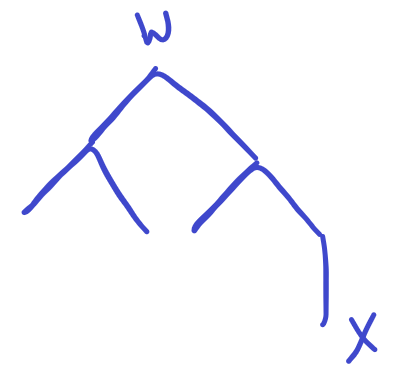
\includegraphics[width = 150pt]{Homework/graph1.png}
\end{center}

If we then choose the farthest point from $w$, this $x$ will be an end node from that graph (if it weren't, then there would be another $x'$ that is further from $w$ then $x$). Run a $bfs(x)$. The tree produced will be a pivoted $bfs(w)$ tree. The reason for this is that there are no cycles in trees (as $G$ is a tree), so there is one unique path between each vertex. The resulting tree will be guaranteed to be fully right leaning, since we have chosen a end node from the $bfs(w)$ graph. Since this tree reflects all the possible paths in $G$, we are guaranteed that the furthest node in a fully right leaning tree is the longest path.

\begin{center}
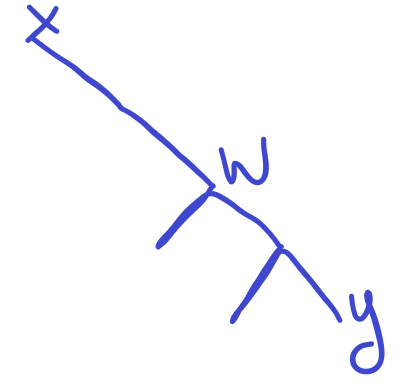
\includegraphics[width = 150]{Homework/graph2.png}
\end{center}

Thus, the procedure outlined above defines how to find the diameter of a tree. 
\begin{flushright}$\blacksquare$\end{flushright}


\end{document}
